\chapter{A kékfestés}
\section{Előzménye és történelmi áttekintése}
Kékfestészet előzményének a kelmefestészetet, és a textilnyomást tartjuk, ami egyszínűre színezést és mintázást jelent mely technológiák már a 15. - 16. században is léteztek. Sok tudást igénylő művészeti ág volt.

A középkori kelmefestés kezdetekben a városokban és a kolostorokban működtek különféle anyagok színezésével foglalkoztak, mint például gyapjú vagy vászon. 

Az indigó megjelenéséig Magyarországon a kelmefestésre a festő csülleng növényből elő- állított kék festékanyagot használták. Ez a 15.században  kerül Magyarországra és terjedt el fő alapanyagként.

A csülleng fontos szerepet töltött be a középkortól kezdve, legnagyobb termelő területek Franciaország és Türningában volt. A magyarországi mestereknek a beszerzési központ Türnigiában volt.
A 16. század körül körülbelül 300 falu foglalkozott a csülleng termesztéssel Magyarországon. Aki akkoriban a csülleng termesztéssel foglakozott vagyonosabb réteghez tartozott. 

A 17. századra visszaeset a termesztés mert ekkortájt a holland hajókaravánok behozták kelet Indiából az indigót.Ezekben az időkben már csak körülbelül 30 falu foglakozott még a termesztéssel.

Az 1600-as évek körül Brassó város könyveiben jelent meg az első feljegyzés a posztó kereskedelemről.
Létezett egy céhen kívüli szervezet aki szétosztotta a mesterek között festendő posztót \cite{domonkos1981magyarorszagi}(14-17).
Miután a mesterek elkészültek a festetett mintás anyagokkal azokat a céh újra összegyűjtötte és kereskedtek velük más városokban vagy exportálták Európa különböző részeire.

A 16. -17. században az ország még török fenhodltság alá nem esőrészén az ország északi területei hirtelen és hatalmas fejlődés vette kezdetét.
Az elfoglalta területekről menekülők elárasztották az ország északi városait és egyre nagyobb lett a zsúfoltság és a népesség, amit az akkori mesterek kihasználtak, de a műhelyek kicsik voltak és a sok munkástól egyre zsúfoltabbá váltak, ez a termelés és a gyártás kárára vált már ekkor.

A kisvárosokban, mint például Lőcse, Eperjes itt már a 16. században több mester fogalakozott anyagok és fonalak
festésével. 

Nem csak a dolgozni vágyó munkások indultak meg a déli országrészről hanem az onan menekülni kényszerülő mesterek is. Ezek a vándorló mesterek új Céheket hoztak létre, bizonyos esetekben a helyi mesterekkel közösen vagy konkurenciaként a már meglévőkkel szemben. 

Az első magyarországi feljegyzés a kékfestésről 1783-bol van Körmöcbányáról, a 17.század közepétől indult meg a kékfestészet elterjedése meghonosodása Magyarországon  %referencia kell erre

A 18. században szinte minden városban volt olyan mesterember, aki ezzel foglalkozott az igen nagy kereslet miatt. Egyre nagyobb kereskedelmi igény alakult ki a nyomot mintás anyagok iránt sok mester próbált új technikákat létre hozni, illetve elsajátítani a más régiókból származókat, hogy ezzel kiemelkedjenek a már meglévő minták és anyagok sokaságából.

Sopronban volt a Boór család, akik a 19. században, az egyik legfontosabb szerepet töltöttek be ők voltak az első mesterek, akik ipari jellegű, gyárszerű  kékfestő üzemet működtettek.
1852 és 1861 között elkezdték a bővítést, és a későbbiekben külföldre is exportálták termékeiket Európa minden pontjára. Hatalmas gazdasági és kereskedelmi előnyre tettek szert a kialakított gyártás technológiának köszönhetően, sokkal alacsonyabb előállítási költséget tudtak elérni. A megnövekedett bevételnek köszönhetően Indiában béreltek földeket ahol saját maguk termesztették indigót.
A Goldberger (Kelenföldi Textilgyár - KELTEX), és a Felmayer (szegedi műhely) is, külföldi tapasztalatok alapján végezte ezeket a munkafolyamatokat a 19. század közepére mindenhol Ipari méretekben ment már a kékfestés és a kelmefestés.
Amikor megtörtént ez a nagy ipari fejlődés a hagyományos manufakturális céhes kisüzemek elkezdtek tönkre menni és ennek a kézműves iparnak a végét jelentette még körü belül 100 évig sikerült fentartanija magát de ezt követően nagyon kis számban maradtak fent műhelyek és mesterek akik a régi technikákat és módszereket tovább tudják adni és tanítani.
Az ipari fejlődés mellette a divat is megváltozott a vidéki életformák változása után a városi dolgozóknak az öltözködésük is meg változott a régi hagyományos viseletek igényei is változni kezdtek Magyarországon.
Az első és a másodig világháború után nyersanyag hiány lépett fel városiasodás tovább csökkentette a műhelyek számát.
De még egy két vidéki helyen ma is foglalkoznak és viszik tovább ezt a mesterséget próbálják fenttartani, hogy ne veszen el a kékfestészetnek a varázsa.

\section{Technológia}
Egy kékfestő műhely létrehozásához is jelentős tőkebefektetésre van/volt szűkség, egy teljesen külön álló épület szükséges hozzá az oka ennek, hogy a kékfestés eljárás során sok veszéjes egymással reagálni képes vegyszert használtak és ezek elkülönítése és tárolása egy fontos igény. Szükséges egy helység a színezésre és a kifőzésre, a  kifőző helységet fekete konyhának hívták nevével ellentétben ez egy álltalában fehérre meszelt sok kádas helységvolt. A minta készítés is egy külön helységeben történik, amit a küpa szobának hívnak. A szárítás általában az udvaron történik, száritó egy az udvar közepén lábakon álló vagy az épület oldalára erősíttet gerendázat (\ref{fig:udvar}. ábra), rosszabb idő esetén ezt akkor bent a műhelyben kell valahogy kivitelezni.

\begin{figure}[h!]
	\centering
	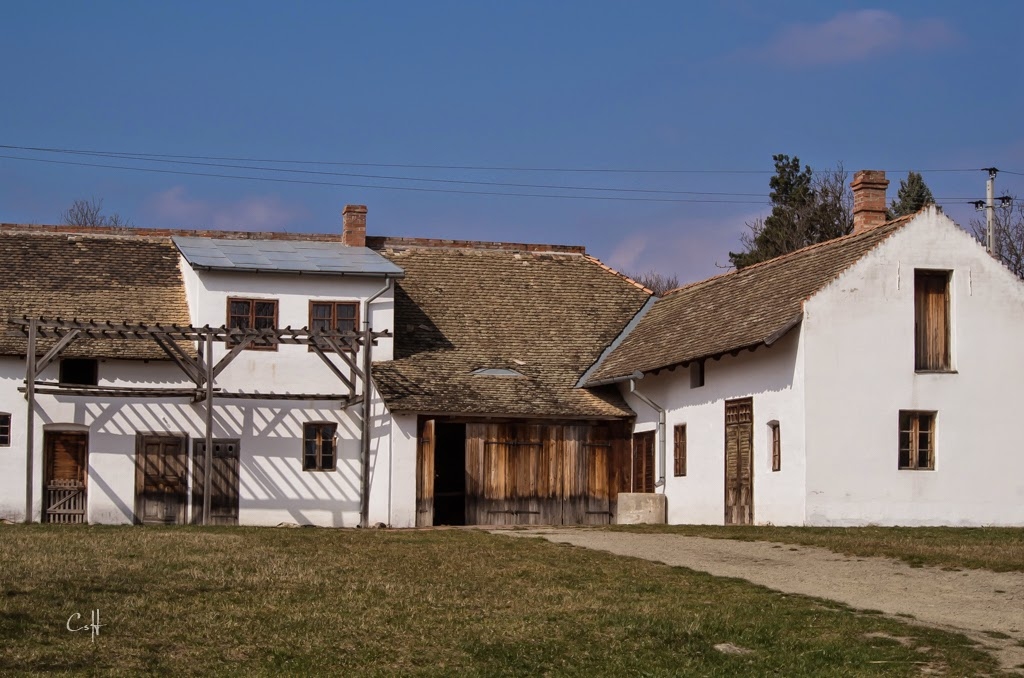
\includegraphics[width=0.5\textwidth]{img/udvar.jpg}
	\caption{Kékfestő műhely , udvar, szárító gerendák}
	\label{fig:udvar}
\end{figure}

Ezek a műhelyek általában a családi telkekre épültek. A az ipari mennyisségben gyártó nagyobb műhelyek kőrű belül 4-5 katlannal rendelkeztek. Az első fő lépés a vásárolt vásznakat kifőzték a szennyeződések miatt, másfél órán keresztül szódás vízben. Miközben ment a kifőzés, keményítős oldalát megjelölték nehogy arra az oldalára kezdjék el a mintázást, mert sajnos akkor az anyagon nem tud rendesen megmaradni a minta és foltos lesz. A fentmaradt végeket a fekete konyhába vitték és egy literes fa kádban tiszta vízben kiöblítették őket. Miután befejeződött a öblítés jött a száritás. A szárítás kültéren vagy beltéren történik attól függően milyen az idő, ha fagyos időben kint száradtak az anyagok akkor a keményítő a hideg hatására elszíneződött és rontotta a végtermék minőségét és esztétikumát az ilyen anyagokat már nem tudták felhasználni és bekerült a selejtek közé, ebben az időszakban szüneteltetniük kellet a munkát ez körű belül 6 hónap kimaradás volt a részűkről. Igy akkor kevesebb munkásra volt szűkségük, de addig az úgy mond pihenő idő alatt sem tétlenkedtek, hanem a minta dúcokat tudták előkészíteni.
A századforduló idejére már több vidéki műhely is rendelkezett gőzgéppel vagy kazánházzal ezeknek a segítségével már betudtak szerelni télire szárítókat a műhelyen belülre is \cite{domonkos1981magyarorszagi}(40-48).
A kézi mintanyomás egy párnázott asztalon készül, amire több rétegben pokrócokat helyeztek majd a végén molinóval befedték, az asztal felületét úgy lehetet elképzelni, mint a pecsét párna lenne, igy az asztal felülete nagyon puha lett.

Búzát, kukoricát, burgonyát alkalmaztak az anyagók keményítésére, ez a folyamat a fekete konyhában történt. A megszáradt végeket elvitték a mángorlóba, ez a szerkezet  egy erős gerendára szerelt asztalalapzatból állt rajta erős vastag keményfa, görgőkön mozgott, mérete körű belül 4-6 méter hosszú lehete és körű belül két és félméter magas, akkoriban ezeket lovakkal hajtották. Kapcsolódott hozzá egy láda, a fölött elhaladt egy főtengely és amire került fel egy vastag lánc, ami az asztalon lévő ládát mozgatta.

A belső kerekeknél két főtengely helyezkedett el váltókar segítségével lehetett irányitani ezzel azt tudták elérni, hogy jobbra és balra is tudták forgatni a szerkezetet. A legfontosabb az volt, hogy kis helyen is elvéghető legyen ez a munka folyamat. A fokozódó verseny helyzet miatt az ipariméretekben gyártókkal olykor előfordult vissza eset a kisműhelyek forgalma és akkor sajnos nem volt pénz lóra, aki hajtsa a kereket akkor maga a mester álltbe és tekerte a szerkezetet. A mángorló több változta is létezik (\ref{fig:mangorlo}. ábra) az általános méret 30x30  ezeket a szerkezetek általában vastag gerendákból építették fel 15-20mm vaslemezeket szereltek fel rá.
Azokba a műhelyekben, ahol adott volt a gépesítés ott gőzgép vagy transzmissziós tengelyekkel vitte az erőt a mángorlóba ezt a technológiát Pápán, Csornán és  Békéscsabán használták.

\begin{figure}[h!]
	\centering
	\begin{subfigure}[b]{0.2\linewidth}
	  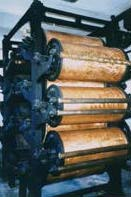
\includegraphics[width=\linewidth]{img/mangorlo.jpg}
	  \caption{}
	\end{subfigure}
	\begin{subfigure}[b]{0.3\linewidth}
	  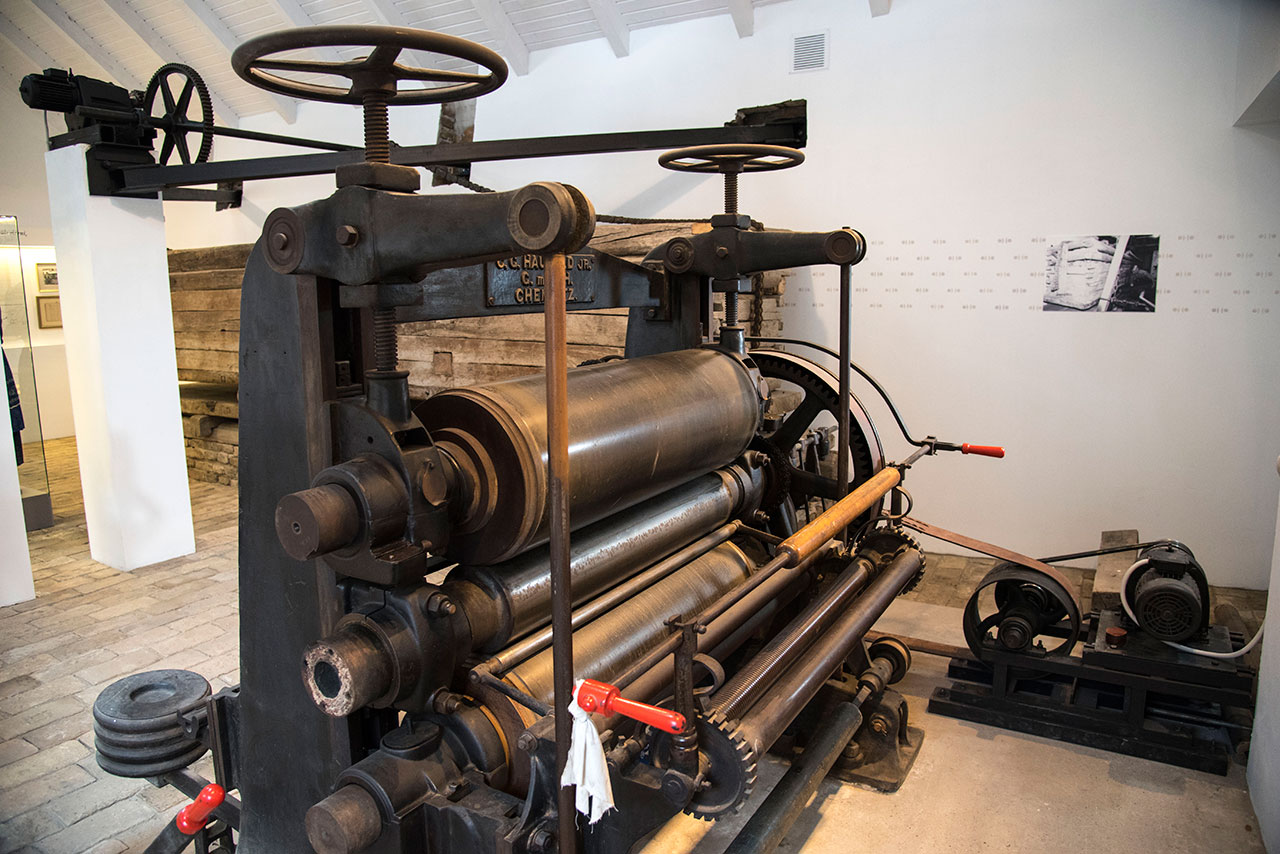
\includegraphics[width=\linewidth]{img/20.jpg}
	  \caption{}
	\end{subfigure}
	\begin{subfigure}[b]{0.3\linewidth}
		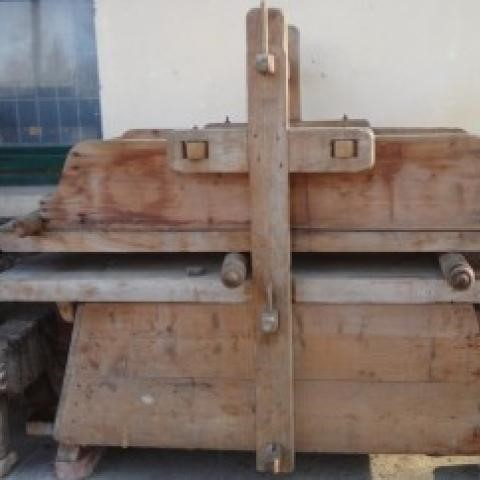
\includegraphics[width=\linewidth]{img/28613.jpg}
		\caption{}
	  \end{subfigure}
	\caption{Mángorlók}
	\label{fig:mangorlo}
  \end{figure}

Más városokban például Bátaszék, előfordult a technikai fejlődésnek köszönhetően, hogy benzinmotort alkalmaztak, vagy mint például Csornán villany meghajtásura építettek át a mángorlót. Fontos fő alkatrésze a mángorlásnak a görgő és az áruhenger volt. Az únt felhelyezték a felsodrószékre és a vászon végét beburkolták. Miközben mozgásban volt nagy súly volt rajta, és ide oda mozgott eközben kisimította az anyagot. Mielőtt elkezdődött a mintázás kétszer háromszor végezték el ezt a folyamatot, a festés után a keményítés körű belül hat - nyolc  vagy akár tíz alkalommal is elvégezték. Maga a mángorló téglával lerakott helység volt itt készítették el a vegyszereket is. 
A minta készítésnél használt fő fedőanyag, az a pap volt álltlában más - más összetételben készült ez anyag nagy titkos receptek alapján készítették el és, hogy több hónapig elegendő legyen így egyszere egy nagy mennyiséget készítettek el.  Ahhoz,hogy ne mennyen tönkre ez az anyag nyirkos hűvös helyen tartották. A papot különböző  pácokhoz és fedőanyagokhoz is hozzá keverték, mikor megkezdődött a kék festés akkor mész lúgos öblítéssel sárga, zöld, narancs színű mintákat is tudtak előállítani.

Nálunk nem volt megszokott a színes mintás anyagok készítése mi maradtunk fehér minták létrehozásánál, ez a stílus inkább a franciák körében volt jellemzőbb. A mintázáshoz is volt egy külön helység, amit használtak és ott abban a helységben volt a tarkázó asztal, ez mellet helyezkedett el a Sasi.
A Sasi egy olyan láda volt, ami körülbelül 6-8 cm mélységű volt, és egy sűrű keményitő oldat volt benne. A ládában volt egy keret aminek ez egyik oldala viaszos vászonnal volt bevonva a másik része pedig monílóval, ebben kenik el a fedő masszát a papot és kürűl belül úgy működik, mint a pecsét párna.
A minta készítés nyomódúcokkal folyt, méret különbségek voltak a dúcok között, de ahhoz hogy hatékonyabb legyen mintás anyagok készítése nagyobb dúcokra kellet válltani de azoknak az elkészítési ideje sok időt vett igénybe igy átváltottak egy úgy nevezett perrotingépre ami  felgyorsította a gyártást. Az 1860 -as évek körül bekövetkezett egy nagy mértékű gépiesítés igy egyre több műhely állt át a gépi nyomásra.

\subsection{Folyamat}

A kékfestészet munkafolyamata úgy zajlott le egy műhelyben, hogy a nyersanyagot nem maguk állítottak elő hanem magánszemélytől vásárolták,vagy maga a megrendelő vitte magával, eztkövetően a megrendelő kiválasztotta a mintát a minta könyvből. 
Voltak olyanok, akik nem foglalkoztak mással mint a nyers alapanyagokat szerezték be a festő mestereknek.

Az első fő lépés az alap vászonnak a megtisztítása, ez egy kétórás folyamat, ami alatt a szövetett egy szódás vizben mossák ki. A szódás kifőzést során az anyagból kioldódik egy gyantás anyag, ami meggátolná a meg színezést és ez a folyamat után az anyag még ki is kifehéredik.

A mosást követi a hideg vizes öblítés és a szárítás ezek a folyamtok néhány órát igényelnek \cite{kisteleki}(107-113).
A száradást követően kap a már tiszta fehér anyag egy vékony keményítést, ami előkészíti a mintázáshoz vagy más éven "tarkázáshoz".

Tarkázásnak említett kézi minta készítés párnázott asztalon készül.

Az asztal mellet helyezték el Únt és az ún-ba mártották bele a minta dúcokat.

A viaszkosvászon belső felületére kent fel a mintaázó pépet az Ún ládát feltöltötték sűrű keményitővel, ami a sasit puhán tartotta. Amit általában használunk hozzá fehér nyomó pép, annak alkotórészei ólom-nitrát, ólomacetát, gumiarábikum, kék timsó, rézgálic. Ezeket össze főzik és miután ki hűlt egy hétre rá használják csak fel. A festék pépet maga a mester szokta elkészíteni általában ez a festék pép akár évekig is elég szokott lenni. A mesterek azt gondolják, hogy egy pép minél régebbi annál fehérebbé teszi a mintát.

A kékfestő a minta dúcot a nyomópépbe nyomja, majd és a dúcot a vászonra illeszti pontosan nehogy elcsúszon és erősen lenyomja, hogy minden pontra kerüljön a pépből és azt a részt nem fogja be a kék indigófesték. A mintázás nagy figyelmet és türelmet igényelt. Általában a kékfestők, 120-130 méter anyagot mintáztak meg, de az napi 13-14 órás munka folyamat \cite{kisteleki}(107-113).
Miután a minta nyomás befejeződött pár nap volt még megszáradt a nyomatás ezek után következet a festés.
Az anyagot egy ráfra akasztják,ami egy vaskerék és erre akasztják fel az anyagot. Ez tehát úgy néz ki az anyag esése miatt mintha vaskereken egy rakott szoknya lenne.
Következő teendő pedig, hogy elkezdték belengedni az indigó festékkel teli kádba és félóránkként fel és le mozgatják az anyagot, és körülbelül 5 - 10 percet hagyják a levegőn, hogy az indigó oxidálódjon.
Amikor elsőnek felhúzzák az anyagot a festékből akkor először egy sárgás - zöld színe van egy kis idő múlva a levegő oxidáló hatására miatt egyre sötétebb zöld színe lesz az utolsó előtti merítés után már világos kék színe van. Miután egyre többet éri a levegő megkapja azt a szép sötétkék színt. amit indigó kéknek nevezünk. 

Miután az anyag elérte a kívánt színt akkor következik a száritás. Miután meg száradt az anyag akkor kap egy kénsavas fürdőt ennél a folyamatnál az történik, hogy kioldódióik a mintázásnál bele ragadta nyomópép és ezek után nagyon szépen elő jön a minta. Utána egy sima vízben is ki öblítik és hagyják megszáradni, és végül ki keményítik az anyagot.

Ez a teljes munkafolyamat valósítja meg azt a fajta mély indigó kék szint ami lehetővé teszi a kontrasztot a minta és a festés között.


%\section{A természet, mint inspiráció}
\section{Minta dúcok}
Maga a minta és a forma készítés rajztudást igényelt és a textilnyomáshoz való ismereteket, a mintáknak mindig pontosan kellett egymáshoz illeszkedniük, ezt a készítőnek mindig szemelőt kellett tartani.

A nyomódúcok felületei általában mindig kiemelkedtek és negatívba kellett rajtuk a mintákat elkészíteni. Két fajta minta dúcot különböztetünk meg, az egyik fából kifaragott a másik pedig réz lemez formájú mintát. A mintadúc készítésének első lépése az, hogy ha fából faragják ki a mintákat akkor kirajzolják a mintafára és utána azt elkezdik kifaragni. 

A kezdetekor úgy nevezték a kézi minta rajzokat, mint például ágas, ágasindás, ágasvirágos, csokros, cakkos, folyondár, margarétás, négyzetpontos,akkoriban nagyon egyszerű neveket adtak a kész mintáknak. A kedvenc és bevált mintákat, idomait a perotinra a mintázó gép nyomó fáira is átvitték (\ref{fig:perotin}. ábra).

\begin{figure}[h!]
	\centering
	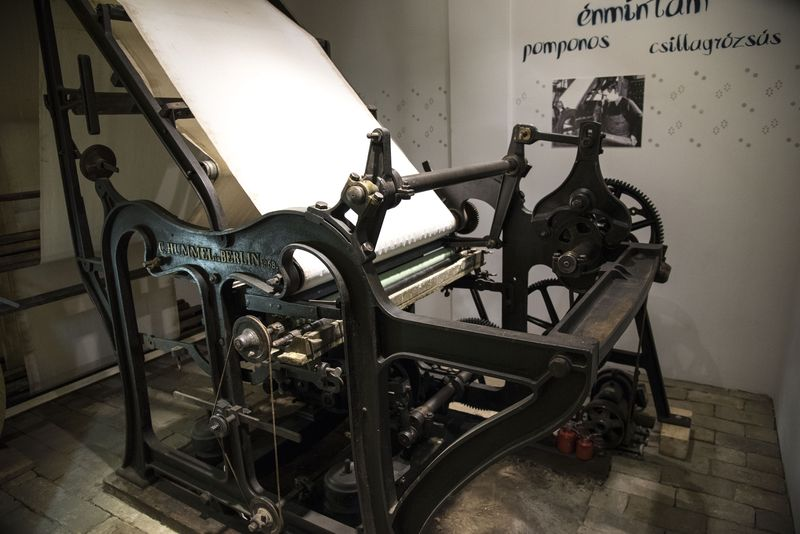
\includegraphics[width=0.5\textwidth]{img/201603-perrotin.jpg}
	\caption{Perotin}
	\label{fig:perotin}
\end{figure}

A 17. század és a 18. századi minta dúcokon pozitív nyomást alkalmaztak amikor növényi vagy figurális mintákat készítettek ezeket a metszeteket fadúcokra készítették. Ebben az időszakban már szinte minden városban volt egy minta készítő mester.

A 18. század közepe táján csak a Sasvári, a Cseklésziek minta készítő műhelyek vagy másnéven manufaktúrák  voltak az országban akik több mintakészítő mestert alkalmaztak azért hogy minél gyorsabban el tudják készíteni a mintáikat, a munkások még az itteni munka mellet tudtak foglalkozni vidéki műhelyek mintáival de miután végeztek mentek is vissza. 

Ez időtájt nem csak a hazai mintakészítők voltak jelen, hanem egyes műhelyek külföldről hívatták a mintakészítő mestereket, akiket a mintatervezés idényére elszállásoltak, ezt a luxust csak a gazdagabb műhelyek engedhették meg maguknak, ha a külföldi mester végzett a megbízatásával akkor már ment is tovább a következő megbízóhoz az újjabb munkákért erről olvashatunk \cite{domonkos1981magyarorszagi} (57-67).
Miután egyre jobban elkezdtek terjedni a nyomot kelmék igy vidéki műhelyek mintakincsei is egyre felkapotabbá kezdtek válni.

Későbbiekben létrejött nagyobb gyárak, mint például Goldberger és Spitzer, Gerson és a Szegedi Felmayer ők alkalmaztak mintafaragó és készítő szakembereket.

A legelső minta fák teljes mértékben fából készültek kisebb pontok, ágak, hasonló képen, mint a folt felületek, de ezeknek a készítésére legalkalmasabbnak a dió fát tartották vagy a körte és gesztenye fát mert ezek a fajták nem szálkásodtak egyszerű volt ki faragani belőlük a mintákat, tartósak voltak és nem repedeztek ki a nedvességtől.

A 16. század idején néhány nyomó dúcok kőzött előfordult tölgy és bükk is ezeknek használatával sok változás jött elő ugyan is ezeknél kezdték el használni a réz drótot, de későbbiekben már teljes mértékben vörös réz drótot használtak, azért volt jobb csak a vörös réz drótot használni mert az előállítása olcsóbb volt és így több mintát tudtak elkészíteni (\ref{fig:duc}. ábra).

\begin{figure}[h!]
	\centering
	\begin{subfigure}[b]{0.2\linewidth}
	  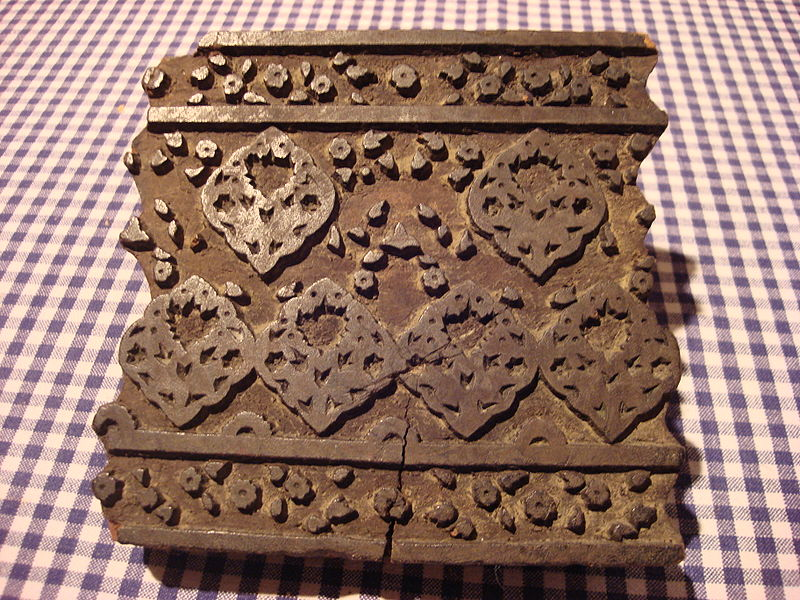
\includegraphics[width=\linewidth]{img/fábolkészült02.jpg}
	  \caption{}
	\end{subfigure}
	\begin{subfigure}[b]{0.2\linewidth}
	  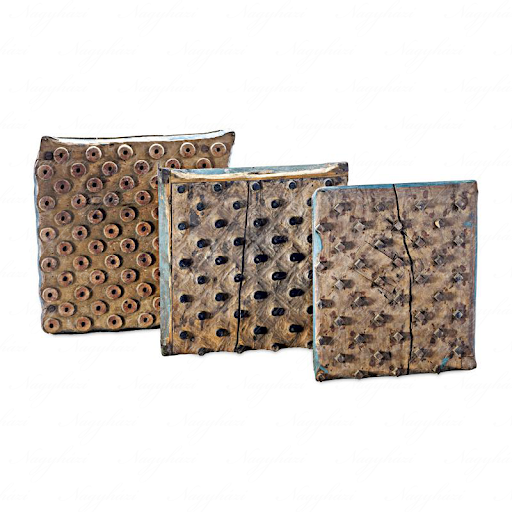
\includegraphics[width=\linewidth]{img/fábolkészült 01.png}
	  \caption{}
	\end{subfigure}
	\begin{subfigure}[b]{0.2\linewidth}
		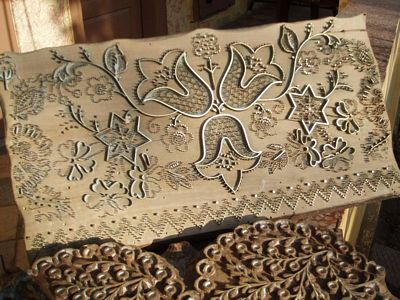
\includegraphics[width=\linewidth]{img/fémbőlkészült.jpg}
		\caption{}
	  \end{subfigure}
	  \begin{subfigure}[b]{0.15\linewidth}
		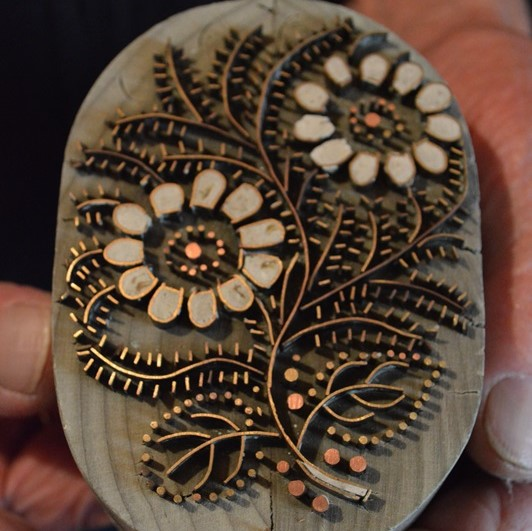
\includegraphics[width=\linewidth]{img/fémből készült 01.jpg}
		\caption{}
	  \end{subfigure}
	\caption{Nyomódúcok}
	\label{fig:duc}
  \end{figure}

%fábólkészült02  %fábolkészült01 %fémbölkészült %fémbölkészult 01
A fémből készített mintáknak a legfontosabb tartozéka az ún volt. A fémből készült minták nagyon időigényesek voltak. A mintákat úgy kezdik el megtervezni, hogy elszőr papír terveket készítenek miután azt elfogadták a mintát elkezdi felrajzolni a minta fára és utána belakozza, hogy miközben készít ne mosódjon el rajt a minta, ritkább vagy bonyolultabb mintáknál a bekarcolják a mintafát, hogy pontosan helyezkedjenek el az elemek.
A minta dúcokra készített mintákhoz lapos vésőt ütögetve haladnak és közben beverik a lemezeket. Ha több szint szeretek volna alkalmazni akkor egy kiegészítő dúcot is készítettek a a kiegészítőmintáról.

Sok festőművész készített ekkor tálytt mintaterveket mit például a békéscsabai festőműhely tulajdonosa Sztaricskay Pál a ki régi kedvenc kézi mintáit elkészítette a gépi nyomáshoz is, aki még  gépi mintákat készített az Gál Gyula volt. Sok esetben ezeket a mintákat csak egy mesternek adták el.

\subsection{Alap és egyébb fő minták}
%egyszerübb pontozott minta
Az öltözködés terén többnyire női ruhákon lehetett látni könnyed és nagyobb, egyszerűbb alap mintákat, formákat, mint például virágók, levelek, apró pöttyök vagy geometrikus formák.
Ezek a minták ugyan úgy rá kerültek ágymenükre zsebkendőre, de terítőn is felehetők voltak.
A természeti motívumok mellet egyre jobban megjelentek és divatossá váltak a geometrikus formák is.
A kezdetekben egyszerű mintákat használtak (\ref{fig:egyszeruminta}. ábra) az idő előre haladtával váltak egyre bonyolultabbá és részletesebb ahogy azt a kor divatja és vevői igényei diktálták.

\begin{figure}[h!]
	\centering
	\includegraphics[width=0.55\textwidth]{img/egyszerübb pontozott minta.jpg}
	\caption{Egyszerű pontozott minta}
	\label{fig:egyszeruminta}
\end{figure}

%levelek01 %virág 01
Fő motívumoknak lehetnek nevezni a kékfestészetben a virág ábrázolásokat vagy valamilyen fajta formáját.  
Ezek a mintaelemek teljes formájukban szoktak megjeleni vagy vonal ábrázolással vagy egy két ponttal ábrázolták ezeket (\ref{fig:levelvirag}. ábra).
A virág ábrázolások jelentése a szeretetett, a hűséget jelképezte és  ezeket a gondolatokat fejezete ki formailag, változatos színvilága sajátos rezgéseket és érzések váltanak ki az emberekből.

\begin{figure}[h!]
	\centering
	\begin{subfigure}[b]{0.4\linewidth}
	  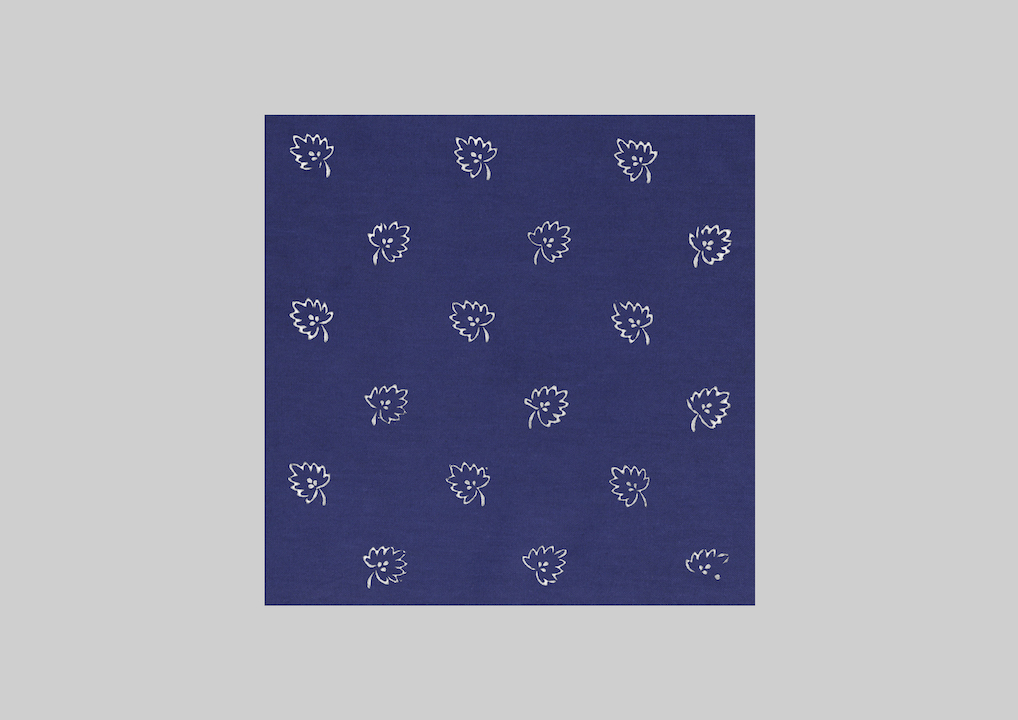
\includegraphics[width=\linewidth]{img/levél01.png}
	  \caption{}
	\end{subfigure}
	\begin{subfigure}[b]{0.43\linewidth}
	  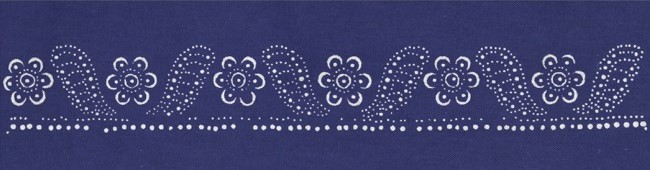
\includegraphics[width=\linewidth]{img/virág 01.jpg}
	  \caption{}
	\end{subfigure}
	\caption{Levél és virág motívumok}
	\label{fig:levelvirag}
  \end{figure}

\subsection{Minta fejlődés}
%sürübb minta 
A Minták olyan irányban fejlődtek tovább, hogy nem csak a már említett egyszerűbb minták voltak hanem elkezdtek más művészeti területekről mintákat beemelni és azokat is tovább fejleszteni (\ref{fig:suruminta}. ábra).
Sokkal nagyon mintafákat készítettek sokkal sűrűbb és aprólékosabb virág, levél motívumokal. Megjelentek a családi címerek is a mintafákon vagy olyan mintát ahol már történtek szerepeltek, mint például vallási jelenetek Ádám és Éva története vagy vadász jelenetek voltak megjelenítve az nem minden esetben volt tiszta hogy igazából miért is jelenítetek meg eseményeket. Pápán a 16. század közepe tájékán készítettek hímzést utánzó kendő mintákat is. A többi városban, mint például Gyula itt damasztszövéshez hasonló minta fát csináltak, Cegléden is az ottani mesterek készítettek szövést és hímzést ábrázoló mintákat.

\begin{figure}[h!]
	\centering
	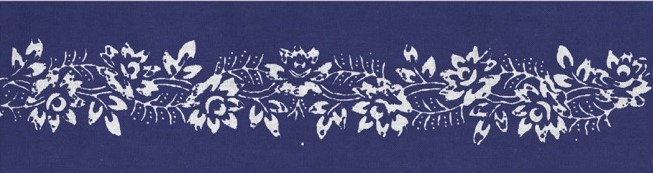
\includegraphics[width=0.55\textwidth]{img/sürübb minta.jpg}
	\caption{Sűrübb minta}
	\label{fig:suruminta}
\end{figure}


\section{Hagyományos kékfestő műhelyek}
A Tolnai Kékfestő műhely Magyarország egyik legrégebbi még ma is működő kékfestő műhely 1810-ben alpítoták.
Műhelyben még fellelhetők a régi eszközök az eredeti hagyományokat követik, még a mai napig a régi eszközökkel dolgoznak.
Motívumaikra jellemző, hogy csak is a régi családi mintafákat használják fel.
Ezekből a minta készletből több mint ötszáz darabbal rendelkezik a család.
Sajnos ezek a darabok nem pótólhatók mert sajnos hazákban évtizedek óta kihalt ez a mesterség, nincsenek már olyan mesterek, akik a minta készítéssel foglalkoznak igy nincs nagyon lehetőség pótolni a tönkre 
ment darabokat.

\section{Kortás megoldások és adaptációk}

\subsection{Polgár Csaba}
Polgár Csaba(Budapest, 1942-03-19, Budapest, 2016-02-11) textílművész munkásságát nagy mértékben befolyásolta a kortárs modern művészet, korszerűséget mindigis komolyan vette, munkáiban előszerettetel mutatta meg a szabadság érzetét \cite{plogarcs}.

\begin{figure}[ht!]
	\centering
	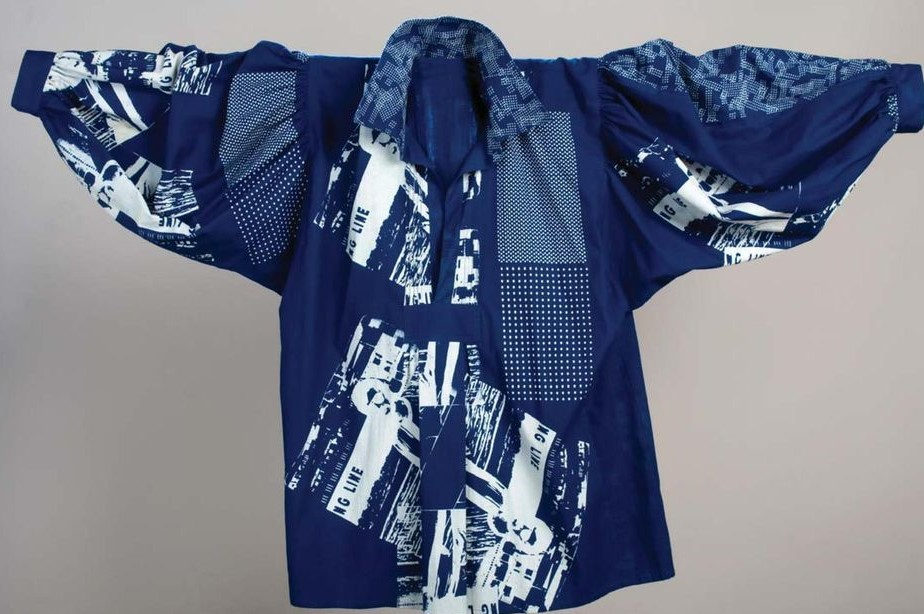
\includegraphics[width=0.55\textwidth]{img/quasi.jpg}
	\caption{Quasi kékfestő program - fényfestésnek - ing}
	\label{fig:quasi}
\end{figure}

Egy új művészeti technológiát fejlesztett ki amit fényfestésnek (\ref{fig:quasi}. ábra) vagy fakításnak nevezett el, ez a technika igazából a fotogramnak a fordítottja, folyamat röviden  a következő lépésekből áll, a festett anyag kikerül a napra akkor veszít a színéből, kitakarásokkal lehet szabályozni, hogy hol fakuljon jobban ezzel külömböző
mintákat hozva létre és a kékre festett alapanyagra dróthálókat teker és így rács szerű mintákat fakít ki belőle.
Az ő nevéhez fűződik a Quasi kékfestő program a programban nem  kékfestő minta dúcokal állitoták elö a mintákat hanem szitával készítették el ezeket a kék anyagokra. Ennek a technikának az alkalmazása teszi lehetővé új textil karakter  létrehozását, de megmaradva a múltbeli alap technikáknál.

\subsection{Horváth Yoshihara Hanga} 
Horváth Yoshihara Hanga japánban élő textilművész fő kutatási területe \cite{hanga2010} a kékfestés hagyományos japán megfelelője a Shibori(\ref{fig:hyh}. ábra).

A munkái során tanulmányozta a növényi festési technikákat itt leginkább az indigóval való festés, színezés lehetőségeit. Kutatása kitért még a termesztési folyamatokra is amit japán tanulmányi uúa során Tokusimában végzett.

\begin{figure}[h!]
	\centering
	\begin{subfigure}[b]{0.3\linewidth}
	  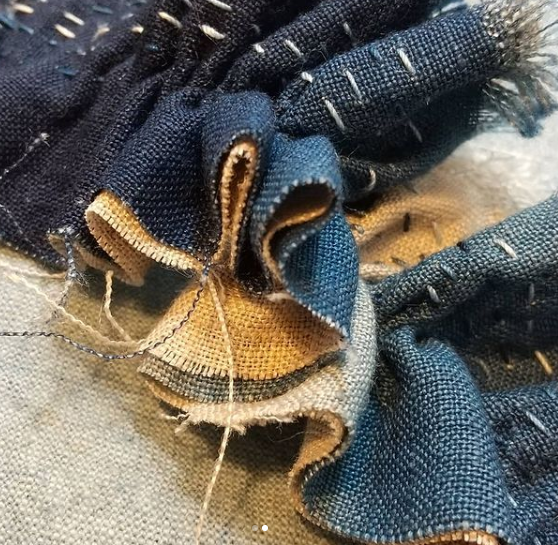
\includegraphics[width=\linewidth]{img/hh_01.png}
	  \caption{}
	\end{subfigure}
	\begin{subfigure}[b]{0.3\linewidth}
	  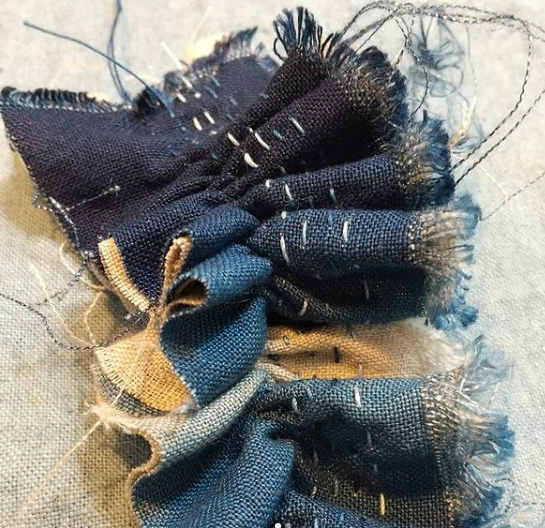
\includegraphics[width=\linewidth]{img/hh_02.png}
	  \caption{}
	\end{subfigure}
	\begin{subfigure}[b]{0.32\linewidth}
		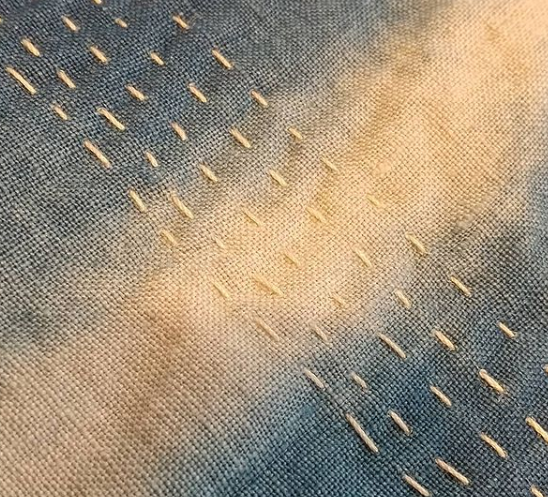
\includegraphics[width=\linewidth]{img/hh_3.png}
		\caption{}
	  \end{subfigure}
	\caption{Horváth Yoshihara Hanga Shibori munkái (forrás:\href{https://www.instagram.com/cicvarek1223}{instagram.com})}
	\label{fig:hyh}
  \end{figure}
\newpage
\subsection{Tóvaj Rozália}

\begin{figure}[ht!]
	\centering
	\begin{subfigure}[b]{0.3\linewidth}
	  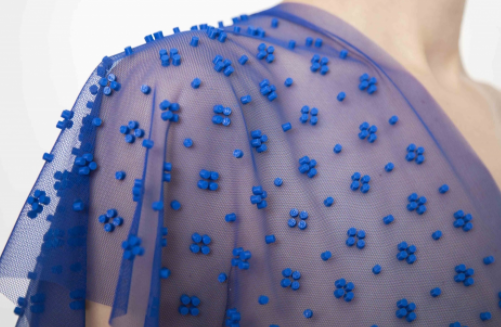
\includegraphics[width=\linewidth]{img/tr_01.png}
	  \caption{}
	\end{subfigure}
	\begin{subfigure}[b]{0.22\linewidth}
	  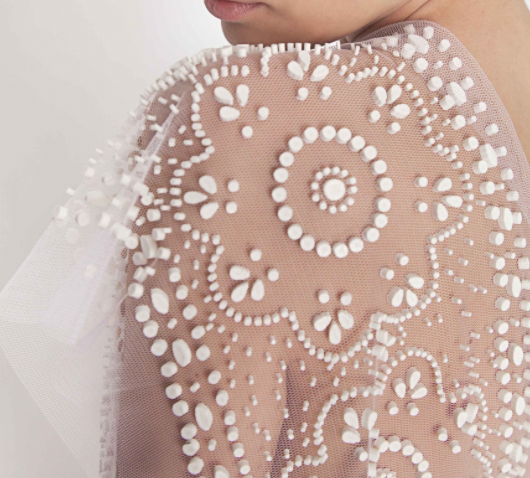
\includegraphics[width=\linewidth]{img/tr_02.png}
	  \caption{}
	\end{subfigure}
	\begin{subfigure}[b]{0.3\linewidth}
		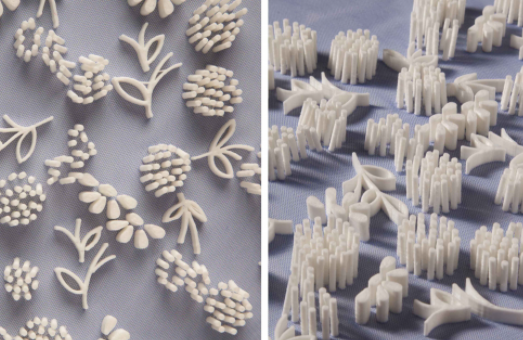
\includegraphics[width=\linewidth]{img/tr_03.png}
		\caption{}
	  \end{subfigure}
	\caption{Tóvaj Rozália 3D kékfestés}
	\label{fig:tr}
  \end{figure}

  Tóvaj Rozália bár a kékfestés hagyományából eredezteti munkáját, egy erős elmozdulás figyelhető meg az alapanyagban és a technológiában. Mestermunkája \cite{tovaj2018} során azzal foglalkozott, hogy újra szerette volna gondolni a hagyományos kékfestést. A célja a gazadag kulturkincs és a mintarendszer tovább vitele a jelenkori technologiákkal. A végső eredmény az lett, hogy a hagyományos mintákat 3D nyomtatással készítette el lágy anyagokra így megidézve a hagyományos formai és minta világot.